\documentclass[../SpecificaTecnica.tex]{subfiles}
\begin{document}
\section{Schema della base di dati}
	\begin{figure}[!h]
		\centering
		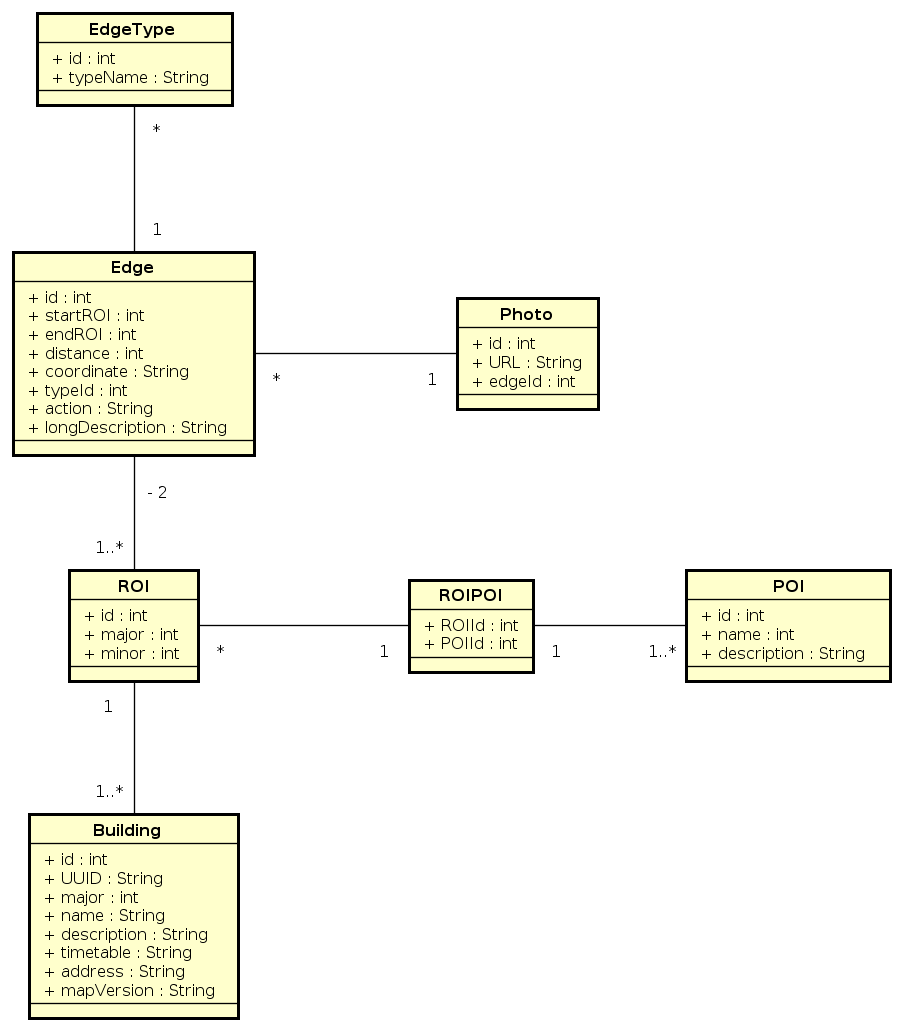
\includegraphics[scale=0.6]{diagrammi/DatabaseSQL.png}
			\caption{Struttura del database}
		\label{fig:Struttura_MVP}
	\end{figure}
	\subsection{Descrizione}
		Il database proposto serve per salvare mappe e informazioni associate ai luoghi in esse contenute. 
	\subsection{Entità}
		\subsubsection{Building}
			Rappresenta un edificio di cui è presente la mappa. I suoi dati sono:
			\begin{itemize}
				\item \textbf{id}: chiave primaria, autoincrementale, intero che identifica univocamente un edificio;
				\item \textbf{UUID}: stringa che rappresenta l'UUID dei beacon utilizzati dal nostro applicativo;
				\item \textbf{major}: intero che distigue i beacon della nostra applicazione appartenenti ad un edificio rispetto a quelli presenti in un altro edificio;
				\item \textbf{name}: stringa che rappresenta il nome dell'edificio;
				\item \textbf{description}: stringa che rappresenta la descrizione dell'edificio(funzione e quialcos'altro);
				\item \textbf{timetable}: stringa che rappresenta gli orari di un edificio;
				\item \textbf{address}: stringa che rappresenta l'indirizzo di un edificio;
				\item \textbf{mapVersion}: stringa che rappresenta la versione della mappa.
			\end{itemize}
		\subsubsection{ROI}
			Rappresenta una ROI all'interno di un edificio. I suoi dati sono:
			\begin{itemize}
				\item \textbf{id}: chiave primaria, autoincrementale, intero che identifica univocamente una ROI;
				\item \textbf{major}: intero che distigue i beacon della nostra applicazione appartenenti ad un edificio rispetto a quelli presenti in un altro edificio;
				\item \textbf{minor}: intero che rappresenta univocamente un beacon della nostra applicazione in un edificio.
			\end{itemize}
		\subsubsection{ROIPOI}
			Rappresenta l'associazione tra ROI e POI. I suoi dati sono:
			\begin{itemize}
				\item \textbf{idROI}: chiave esterna, intero che identifica univocamente una ROI;
				\item \textbf{idPOI}: chiave esterna, intero che identifica univocamente un POI;
			\end{itemize}
		\subsubsection{POI}
			Rappresenta una POI all'interno di un edificio. I suoi dati sono:
			\begin{itemize}
				\item \textbf{id}: chiave primaria, autoincrementale, intero che identifica univocamente un POI;
				\item \textbf{name}: stringa che identifica in qualche modo un POI;
				\item \textbf{description}: string a che spiega le funzionalità fi un POI ed altro.
			\end{itemize}
		\subsubsection{Edge}
			Rappresenta un collegamento tra due ROI. I suoi dati sono:
			\begin{itemize}
				\item \textbf{id}: chiave primaria, autoincrementale, intero che identifica univocamente un POI;
				\item \textbf{startROI}: chiave esterna, intero che identifica univocamente il ROI di partenza dell'edge;
				\item \textbf{endROI}: chiave esterna, intero che identifica univocamente il ROI di arrivo dell'edge;
				\item \textbf{coordinate}: ?intero? ?identifica la rotazione dell'utente per procedere secondo il persorso ideale?;
				\item \textbf{distance}: intero che identifica la distanza tra startROI e ednROI;
				\item \textbf{typeId}: chiave esterna, intero che identifica il tipo di arco;
				\item \textbf{action}: stringa che identifica qualche azione da compiere per attraversare l'arco;
				\item \textbf{longDescription}: stringa che fornisce le le indicazioni dettagliate di attraversamento di un arco.
			\end{itemize}
		\subsubsection{Photo}
			Rappresenta una fotografia di utile per attraversare un edge. I suoi dati sono:
			\begin{itemize}
				\item \textbf{id}: chiave primaria, autoincrementale, intero che identifica univocamente una fotografia;
				\item \textbf{URL}: stringa che rappresenta l'URL al quale è possibile recuperare la fotografia;
				\item \textbf{edgeId}: chiave esterna, intero che identifica univocamente l'edge a cui la fotografia è associata.
			\end{itemize}
		\subsubsection{EdgeType}
			Rappresenta un tipo di edge. I suoi dati sono:
			\begin{itemize}
				\item \textbf{id}: chiave primaria, autoincrementale, intero che identifica univocamente un tipo di edge;
				\item \textbf{typeName}: stringa che descrive il tipo di edge.
			\end{itemize}
	\subsection{Relazioni}
		\subsubsection{Building - ROI}
			\begin{itemize}
				\item \textbf{Tipo di relazione}: 1 a N;
				\item ogni Building può essere associato a 1 o più ROI;
				\item ogni ROI è associato ad un unico Building.
			\end{itemize}
		\subsubsection{ROI - ROIPOI}
			\begin{itemize}
				\item \textbf{Tipo di relazione}: 1 a N (risoluzione della relazione N a N tra ROI e POI);
				\item ogni ROI può essere associato a 0 o più ROIPOI;
				\item ogni ROIPOI è associato ad un unico ROI.
			\end{itemize}
		\subsubsection{ROIPOI - POI}
			\begin{itemize}
				\item \textbf{Tipo di relazione}: 1 a N (risoluzione della relazione N a N tra ROI e POI);
				\item ogni POI può essere associato a 1 o più ROIPOI;
				\item ogni ROIPOI è associato ad un unico POI.
			\end{itemize}
		\subsubsection{ROI - Edge}
			\begin{itemize}
				\item \textbf{Tipo di relazione}: 2 a N;
				\item ogni ROI può essere associato a 1 o più Edge;
				\item ogni Edge è associato a 2 ROI.
			\end{itemize}
		\subsubsection{Edge - Photo}
			\begin{itemize}
				\item \textbf{Tipo di relazione}: 1 a N;
				\item ogni Photo può essere associata ad un unico Edge;
				\item ogni Edge può essere associato a 1 o più Photo.
			\end{itemize}
		\subsubsection{Edge - EdgeType}
			\begin{itemize}
				\item \textbf{Tipo di relazione}: 1 a N;
				\item ogni Edge può essere associata ad un unico EdgeType;
				\item ogni EdgeType può essere associato a 0 o più Edge.
			\end{itemize}
	\subsection{SQL}
		\lstset{language=Pascal}
			\begin{lstlisting}
CREATE TABLE IF NOT EXISTS Building{
	id PRIMARY KEY INT,
	UUID VARCHAR(255),
	major INT,
	name VARCHAR(255),
	description VARCHAR(2000),
	timetable VARCHAR(255),
	address VARCHAR(255),
	mapVersion VARCHAR(255)
}
CREATE TABLE IF NOT EXISTS ROI{
	id PRIMARY KEY INT,
	major INT REFERENCES Building(major),
	minor INT UNIQUE
}
CREATE TABLE IF NOT EXISTS ROIPOI{
	idROI INT REFERENCES ROI(id),
	idPOI INT REFERENCES POI(id),
	PRIMARY KEY (idROI, idPOI)
}
CREATE TABLE IF NOT EXISTS POI{
	id PRIMARY KEY INT,
	name VARCHAR(255),
	description VARCHAR(2000)
}
CREATE TABLE IF NOT EXISTS Edge{
	id PRIMARY KEY INT,
	startROI INT REFERENCES ROI(id),
	endROI INT REFERENCES ROI(id),
	distance INT,
	coordinate INT,
	typeId INT REFERENCES EdgeType(id),
	action VARCHAR(255),
	longDescription VARCHAR(2000)
}
CREATE TABLE IF NOT EXISTS Photo{
	id PRIMARY KEY INT,
	URL VARCHAR(2048),
	edgeId INT REFERENCES Edge(id)
}
CREATE TABLE IF NOT EXISTS EdgeType{
	id PRIMARY KEY INT,
	typeName VARCHAR(255)
}
			\end{lstlisting}
\end{document}